\chapter{Discussion and Comparison}\label{discussion-and-comparison}

\section{Discussion}

\subsection{Reflection directionality}\label{reflection-directionality}

Many objects only become visible when their surface is oriented
perpendicularly to the incident radar waves, so that enough scattered EM
energy makes its way back to the sensor. This is very visible in the
Underground scan, where a glass wall is detected as the robot passes it,
but not while the robot sees it at an angle.

In the Torture Chamber scan, the same effect is visible for chair legs,
especially for the chair at the scene center. the legs appear in clear
form as soon as the radar sees the leg from a point that is orthogonal
to the office chair legs.



\subsection{Material-dependent echo strength}\label{material-dependent-echo-strength}

Some materials, like metal, are obviously better at reflecting radar
waves than others, like Styrofoam. Metal objects cause particularly
strong echos which are visible from a higher distance. This can be
observed in the hallway scans (e.g.~Orbit, Public Restroom, Queue,
Racetrack, Sauna, Underground), where the metal frames of doors and
glass walls stand out in the scan.

\subsection{Doppler vs Direction of Arrival data quality}\label{doppler-vs-direction-of-arrival-data-quality}

In forward-facing geometry (scans D-T), the DOA is necessary to resolve
the sign of a target's reprojection angle. This works fairly well, for
example at the start of Sauna (see \cref{fig:sauna_doa}), the closer target
passes on the right (more pink), while the other targets stay to the
left side of the robot (more green).

\begin{figure}[htbp]
    \centering
    \begin{subfigure}[b]{0.45\textwidth}
        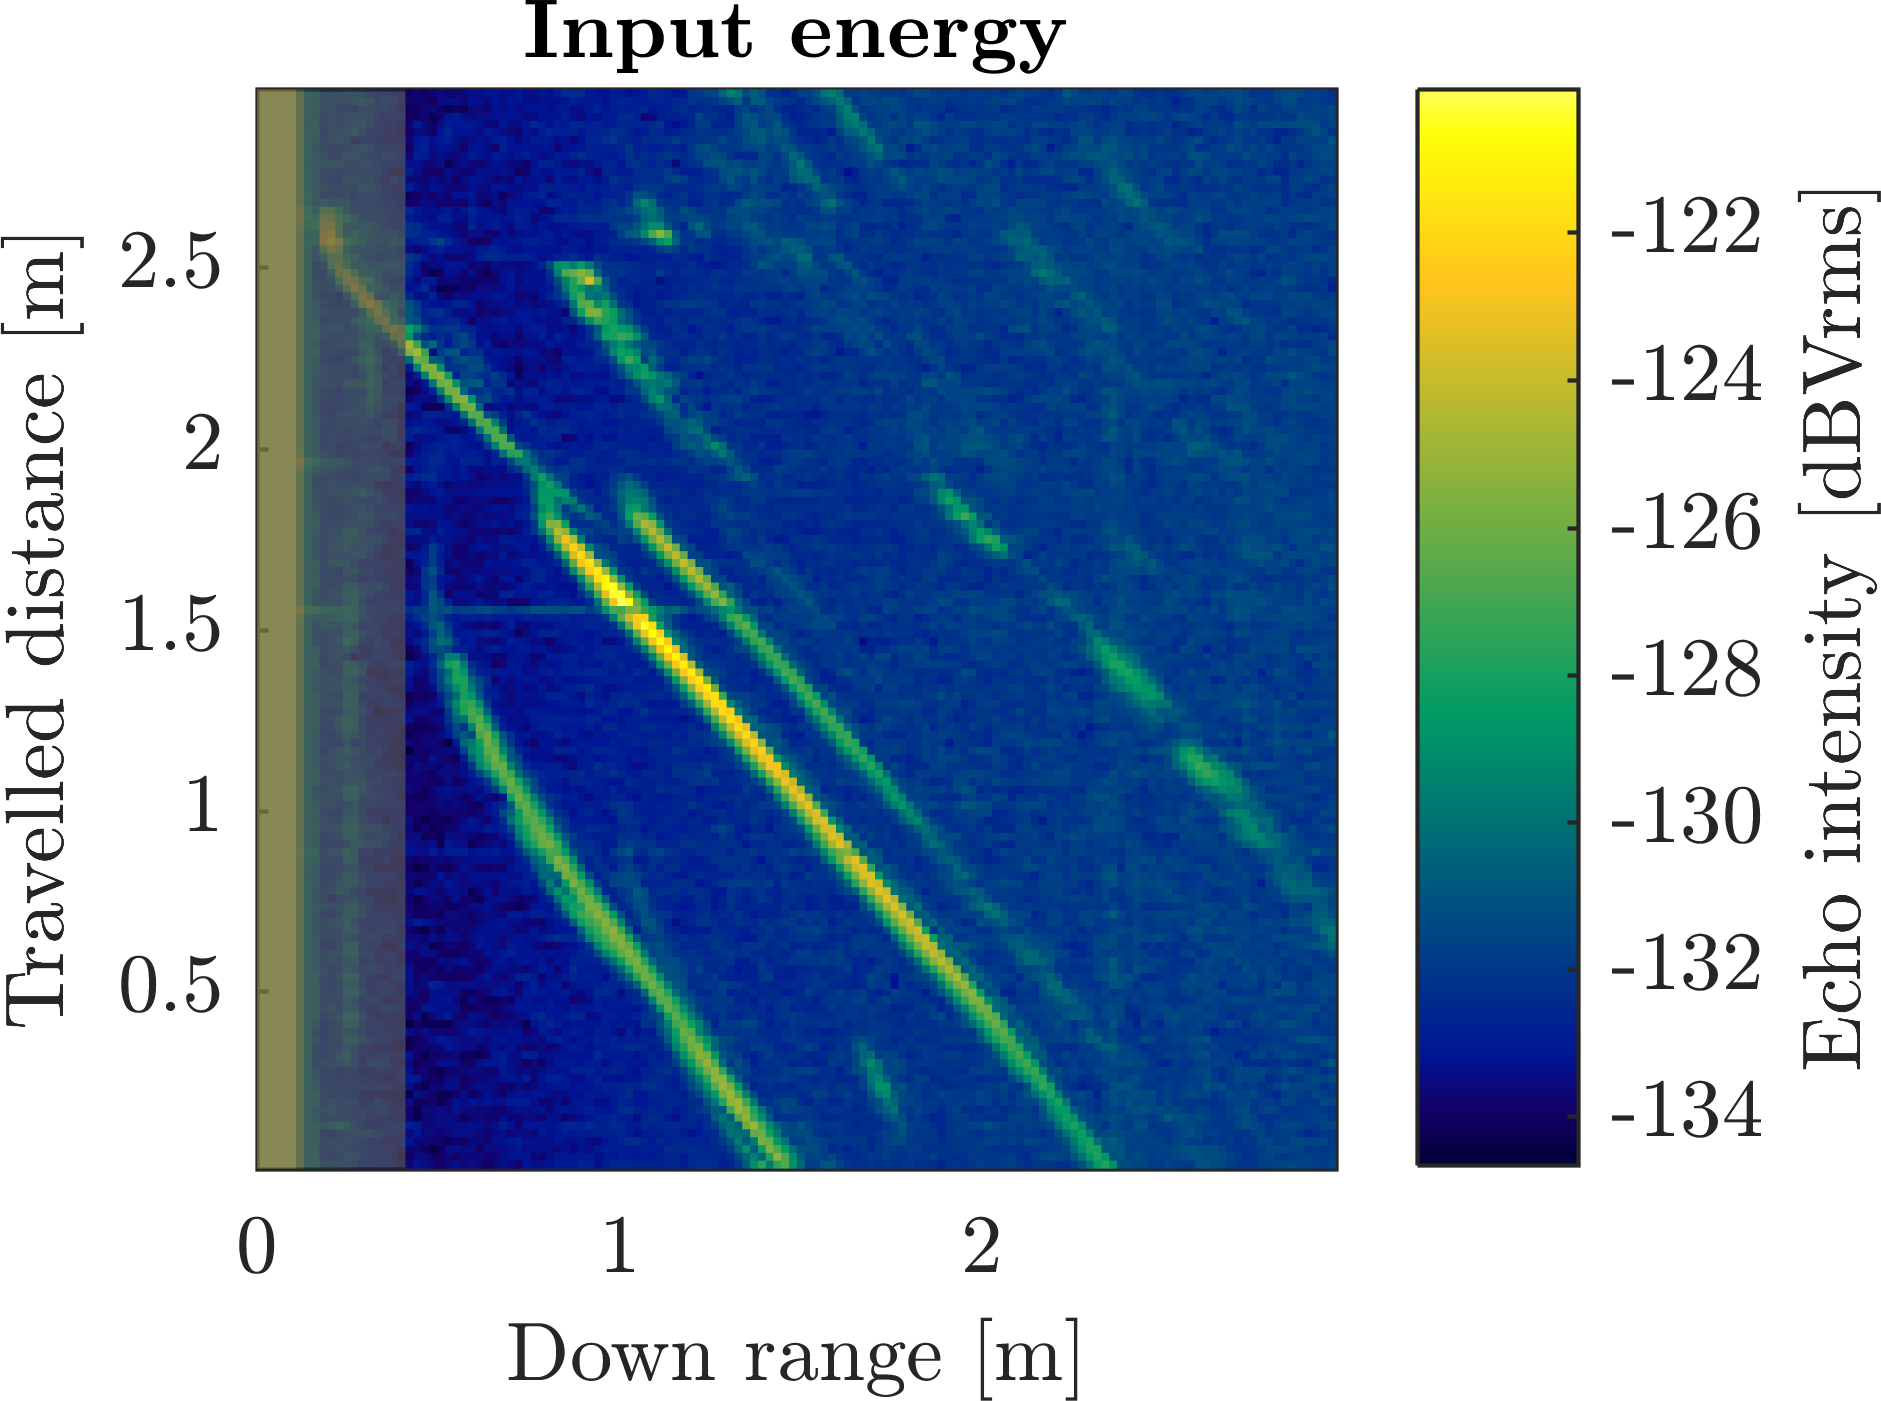
\includegraphics[width=\linewidth]{figures/fig_doa_sign_input.png}
        \caption{\label{fig:sauna_input}Echo intensity}
    \end{subfigure}%
    \hfill%
    \begin{subfigure}[b]{0.45\textwidth}
        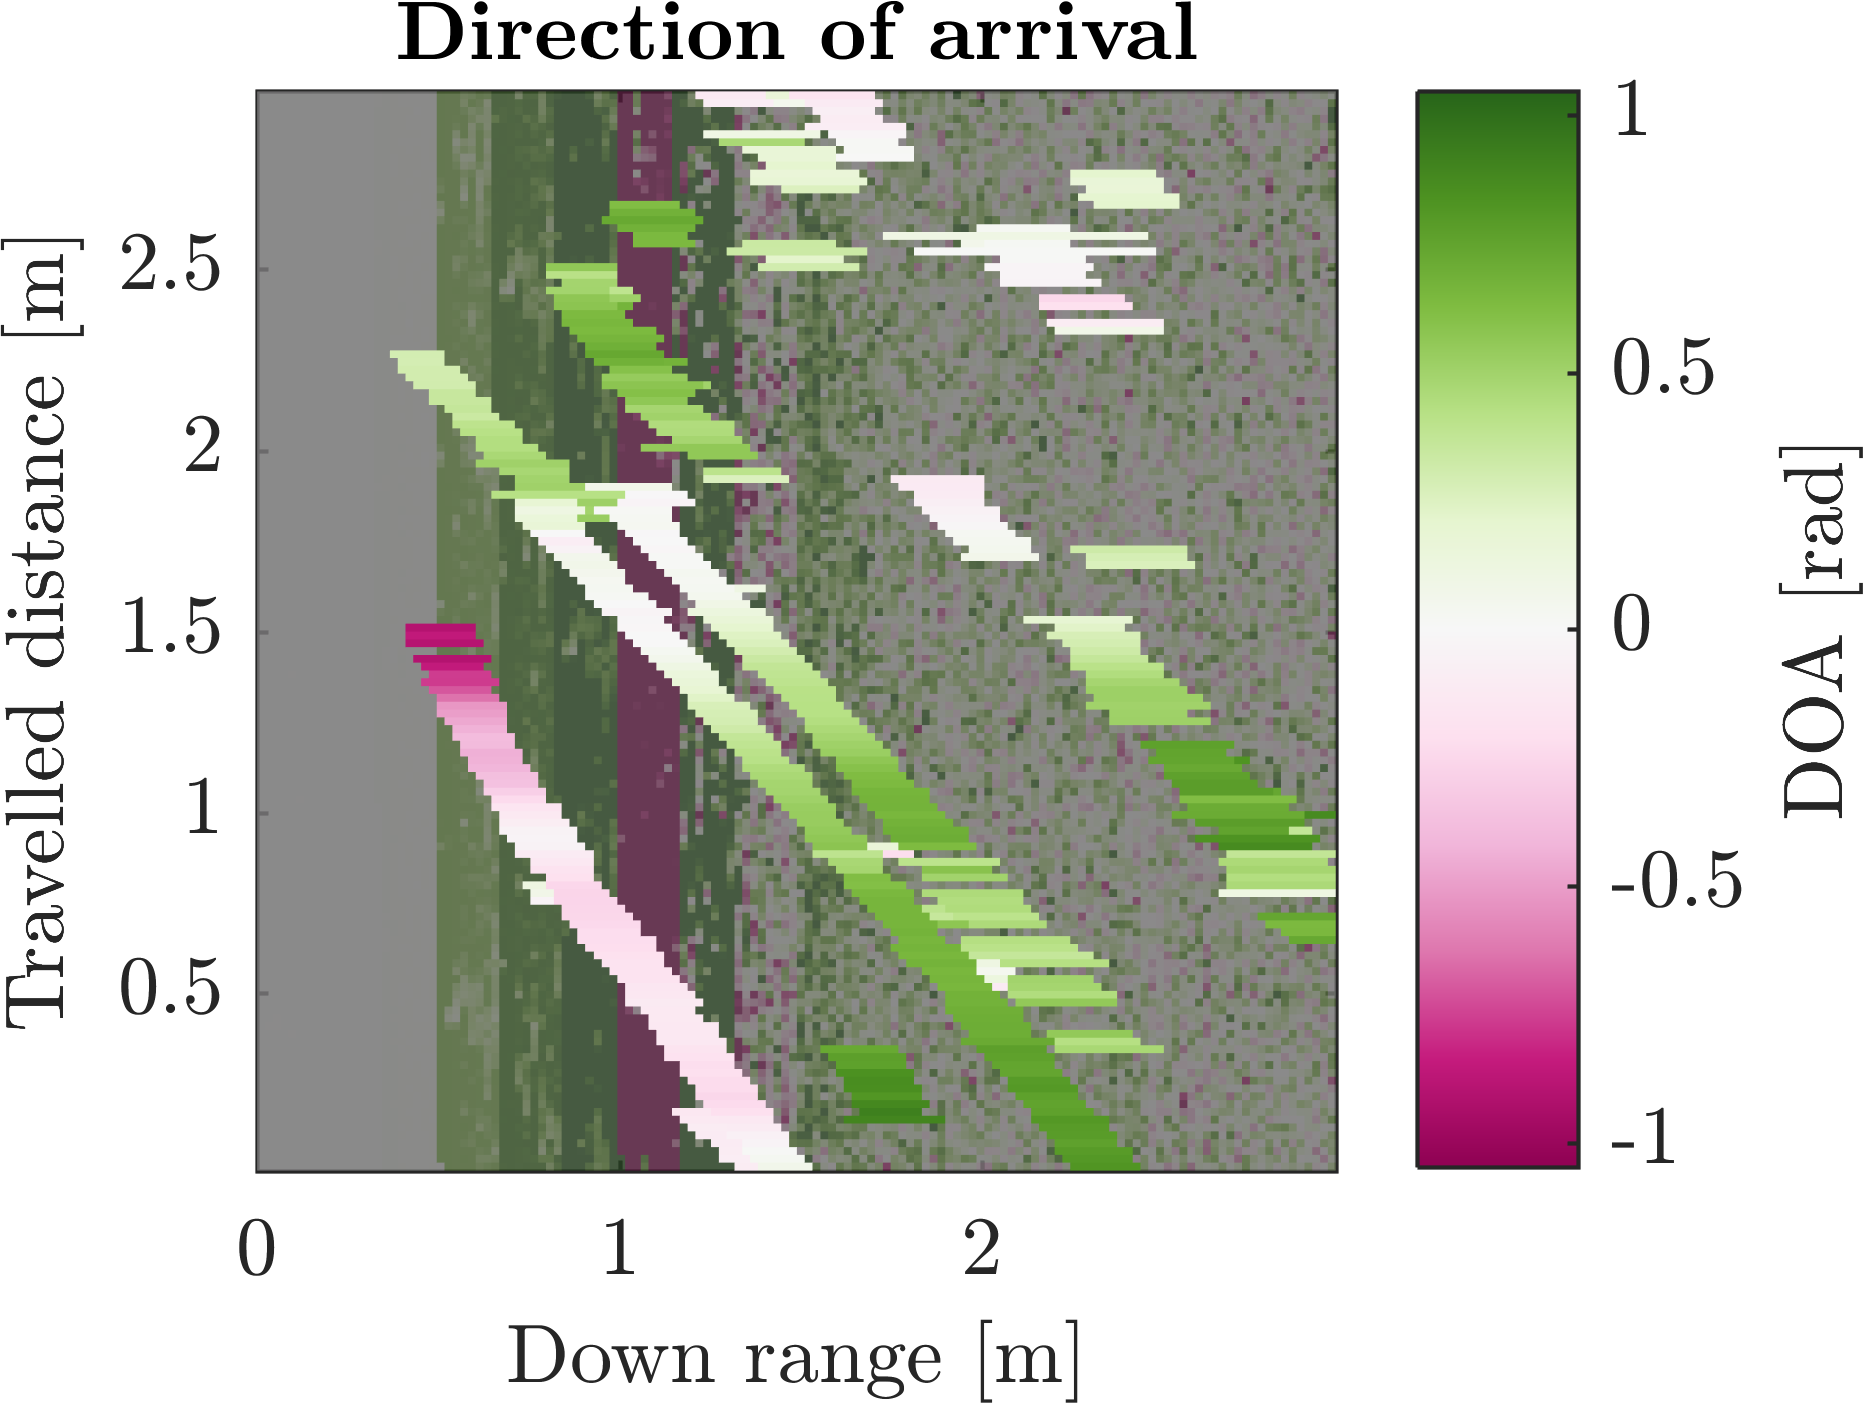
\includegraphics[width=\linewidth]{figures/fig_doa_sign_doa.png}
        \caption{\label{fig:sauna_doa}Direction of arrival estimation}
    \end{subfigure}
    \caption{Range profile and DOA of Sauna scan.}
    \label{fig:sauna}
\end{figure}

In fact, for the side-facing case, the smoothed DOA data also turned out
to be very good. It could even be used to calculate a more precise
reprojection angle.

\subsection{Multipath effects}\label{multipath-effects}

Multipath effects are a well-known problem in ground-based radar
applications \cite{Adams2012}. In situations where multi-path effects
are likely, there is a higher possibility that multiple versions of a
target's echo are visible, which can lead to detection of incorrect
angle and ranges. Luckily, in the recorded data almost no multipath
effects are obvious. The only scan that shows some effects is the
Torture Chamber. There, it seems like the radar waves bounce around a
bit in the (\SI{2}{m},\SI{2}{m}) area under the desk. The effect is that some targets
are detected behind the wall behind the desk.



\subsection{Object penetration}\label{object-penetration}

Some objects are penetrated by the radar waves. For example, in the
Attic and Basement scans, both the front and the back wall of the
plastic bottle can be seen. However, the plastic bottle was relatively
close to the sensor. On the other hand, in the scans with glass walls in
them (P,Q,R,S,U), no significant radar echo is picked up from the
(metal) chair legs behind the glass wall. This is because a typical
glass pane attenuates the \SI{60}{GHz} signal by about \SI{5.5}{dB} \cite{Lu2014}. In
effect, a radar sensor with higher transmission power might be able to
see through walls, but in the conducted experiments radar echos were to
faint to be picked up after the first bigger object (like a wall).

\subsection{Negative obstacles}\label{negative-obstacles}

\begin{figure}[htbp]
% 0.95 * 2832*2268/2124 / (2832*2268/2124 + 3024) = 0.475
% 0.95 * 3024 / (2832*2268/2124 + 3024) = 0.475
    \centering
    \begin{subfigure}[t]{.475\textwidth}
        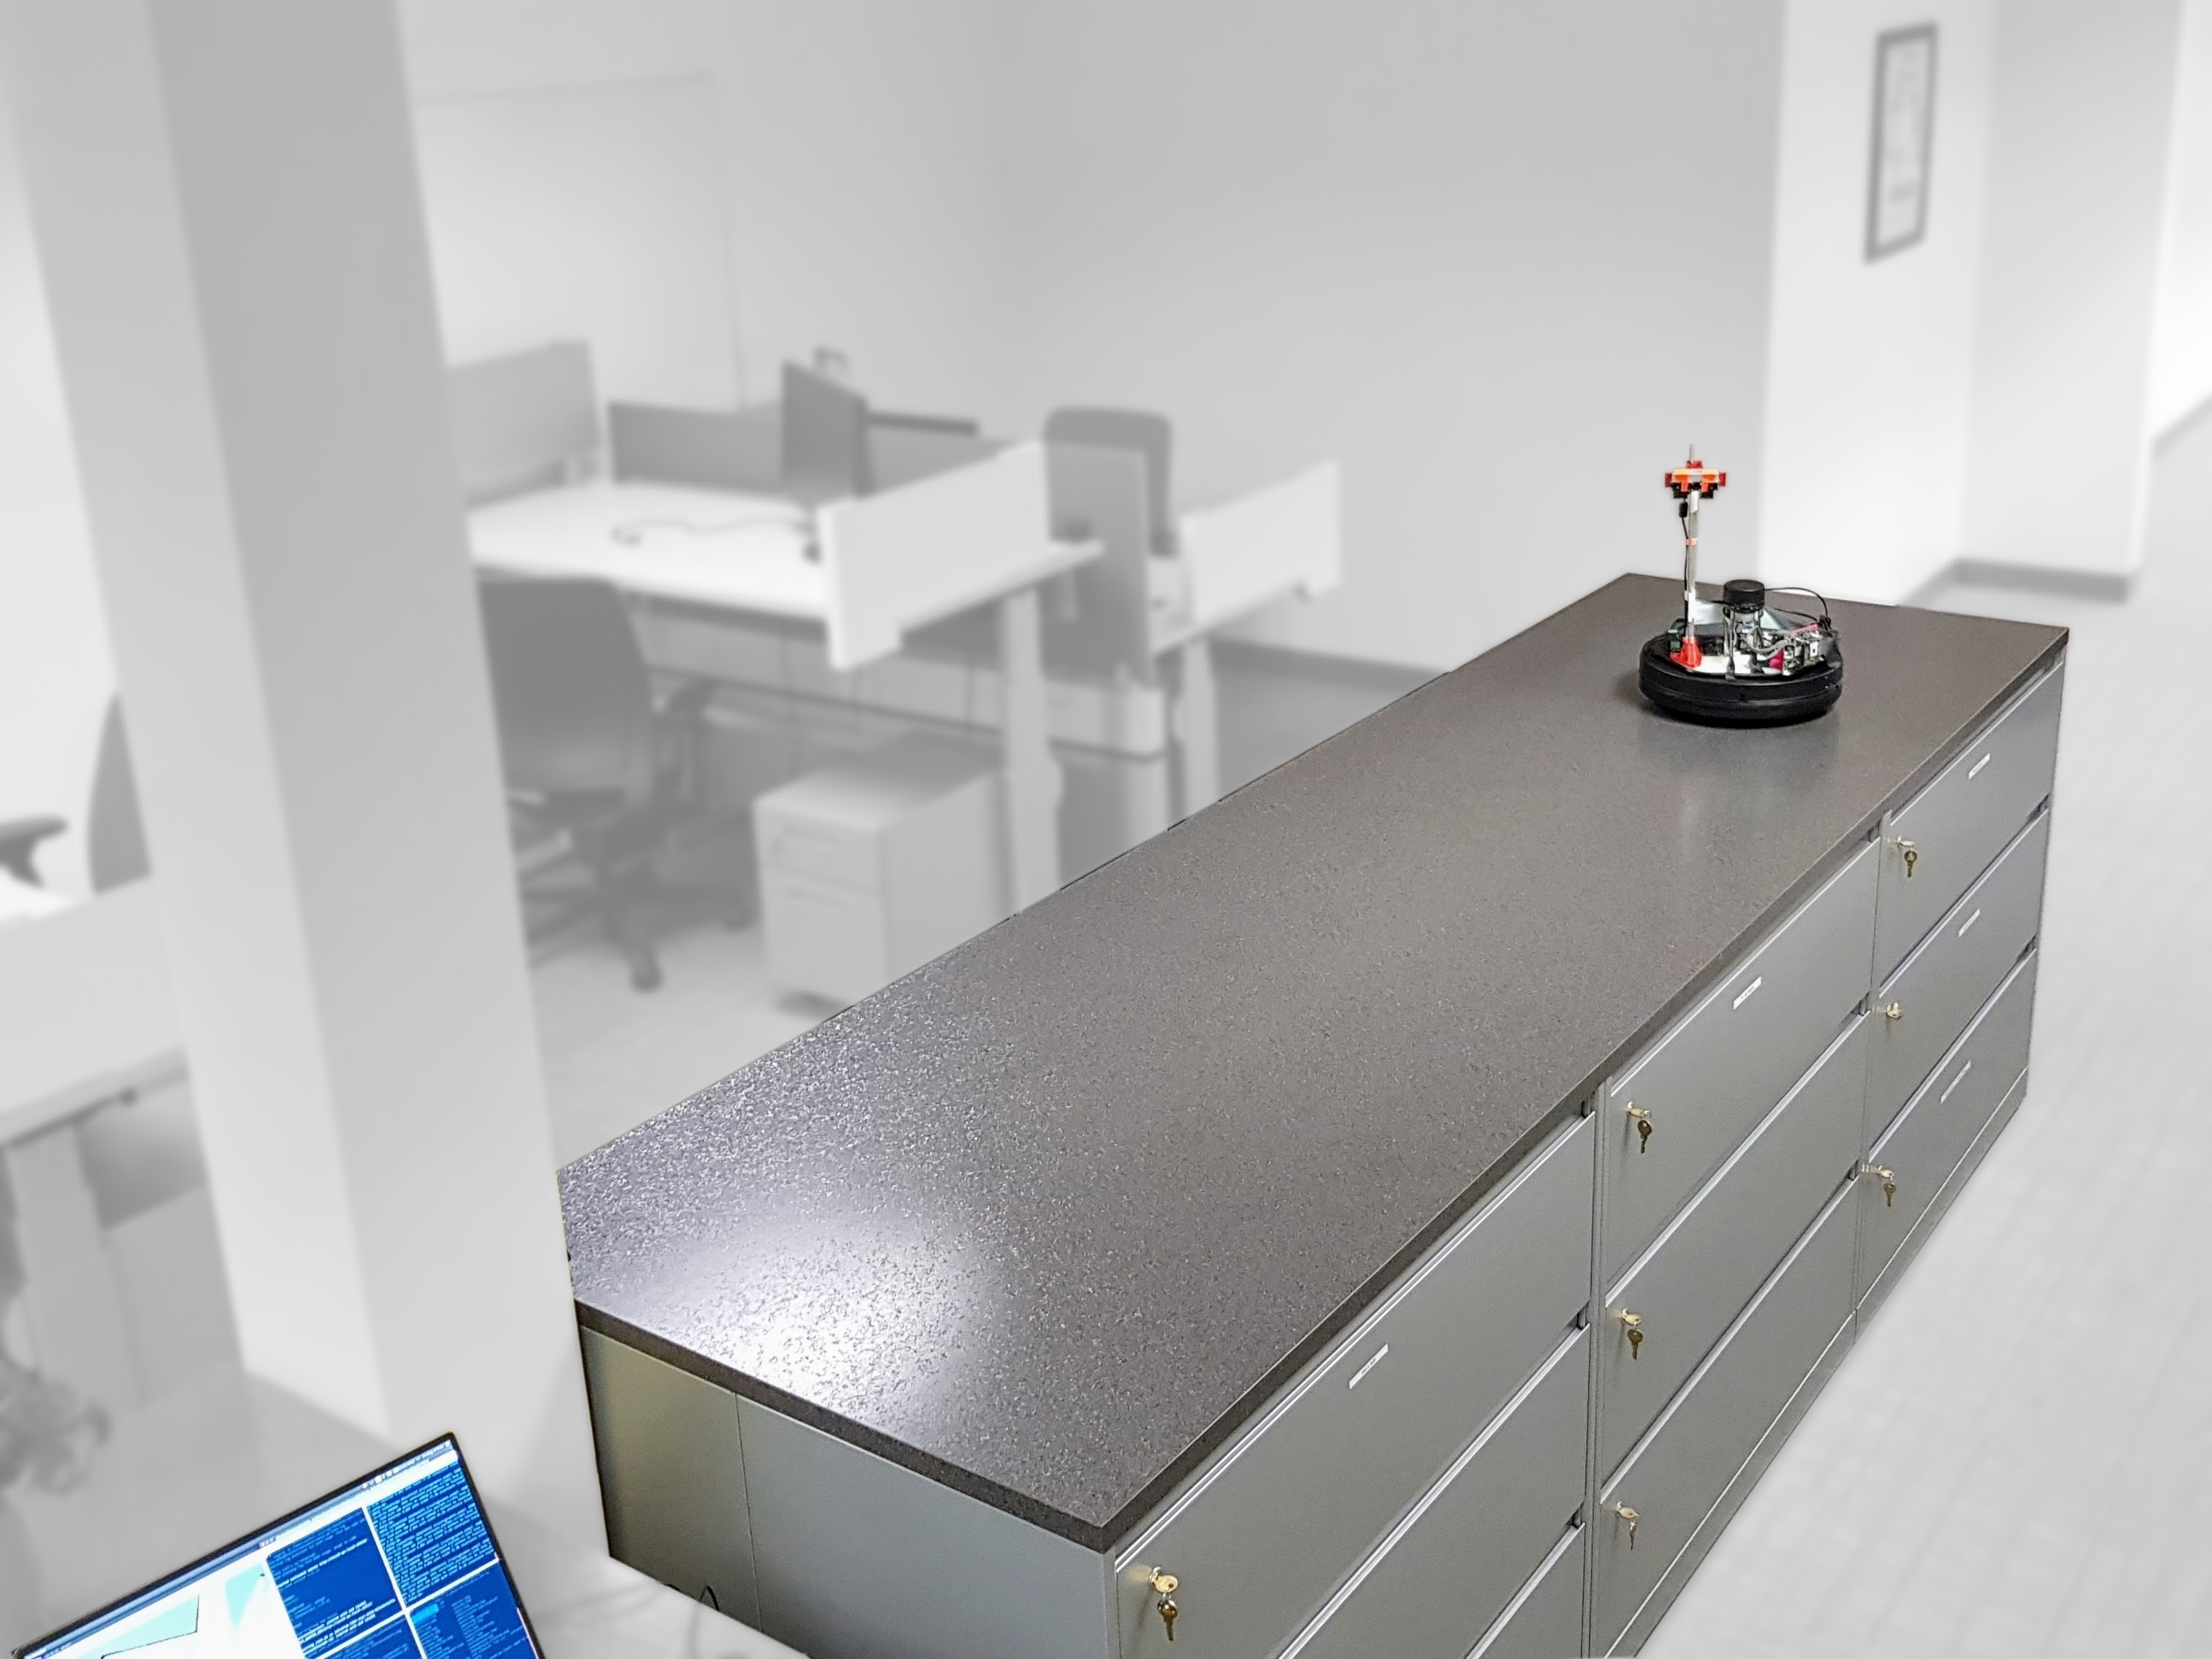
\includegraphics[width=\textwidth]{gfx/pictures/cliff}
        \caption{For the negative obstacle detection tests the robot was driving on the cabinet.}
        \label{fig:cliff}
    \end{subfigure}%
    \hfill%
    \begin{subfigure}[t]{.475\textwidth}
        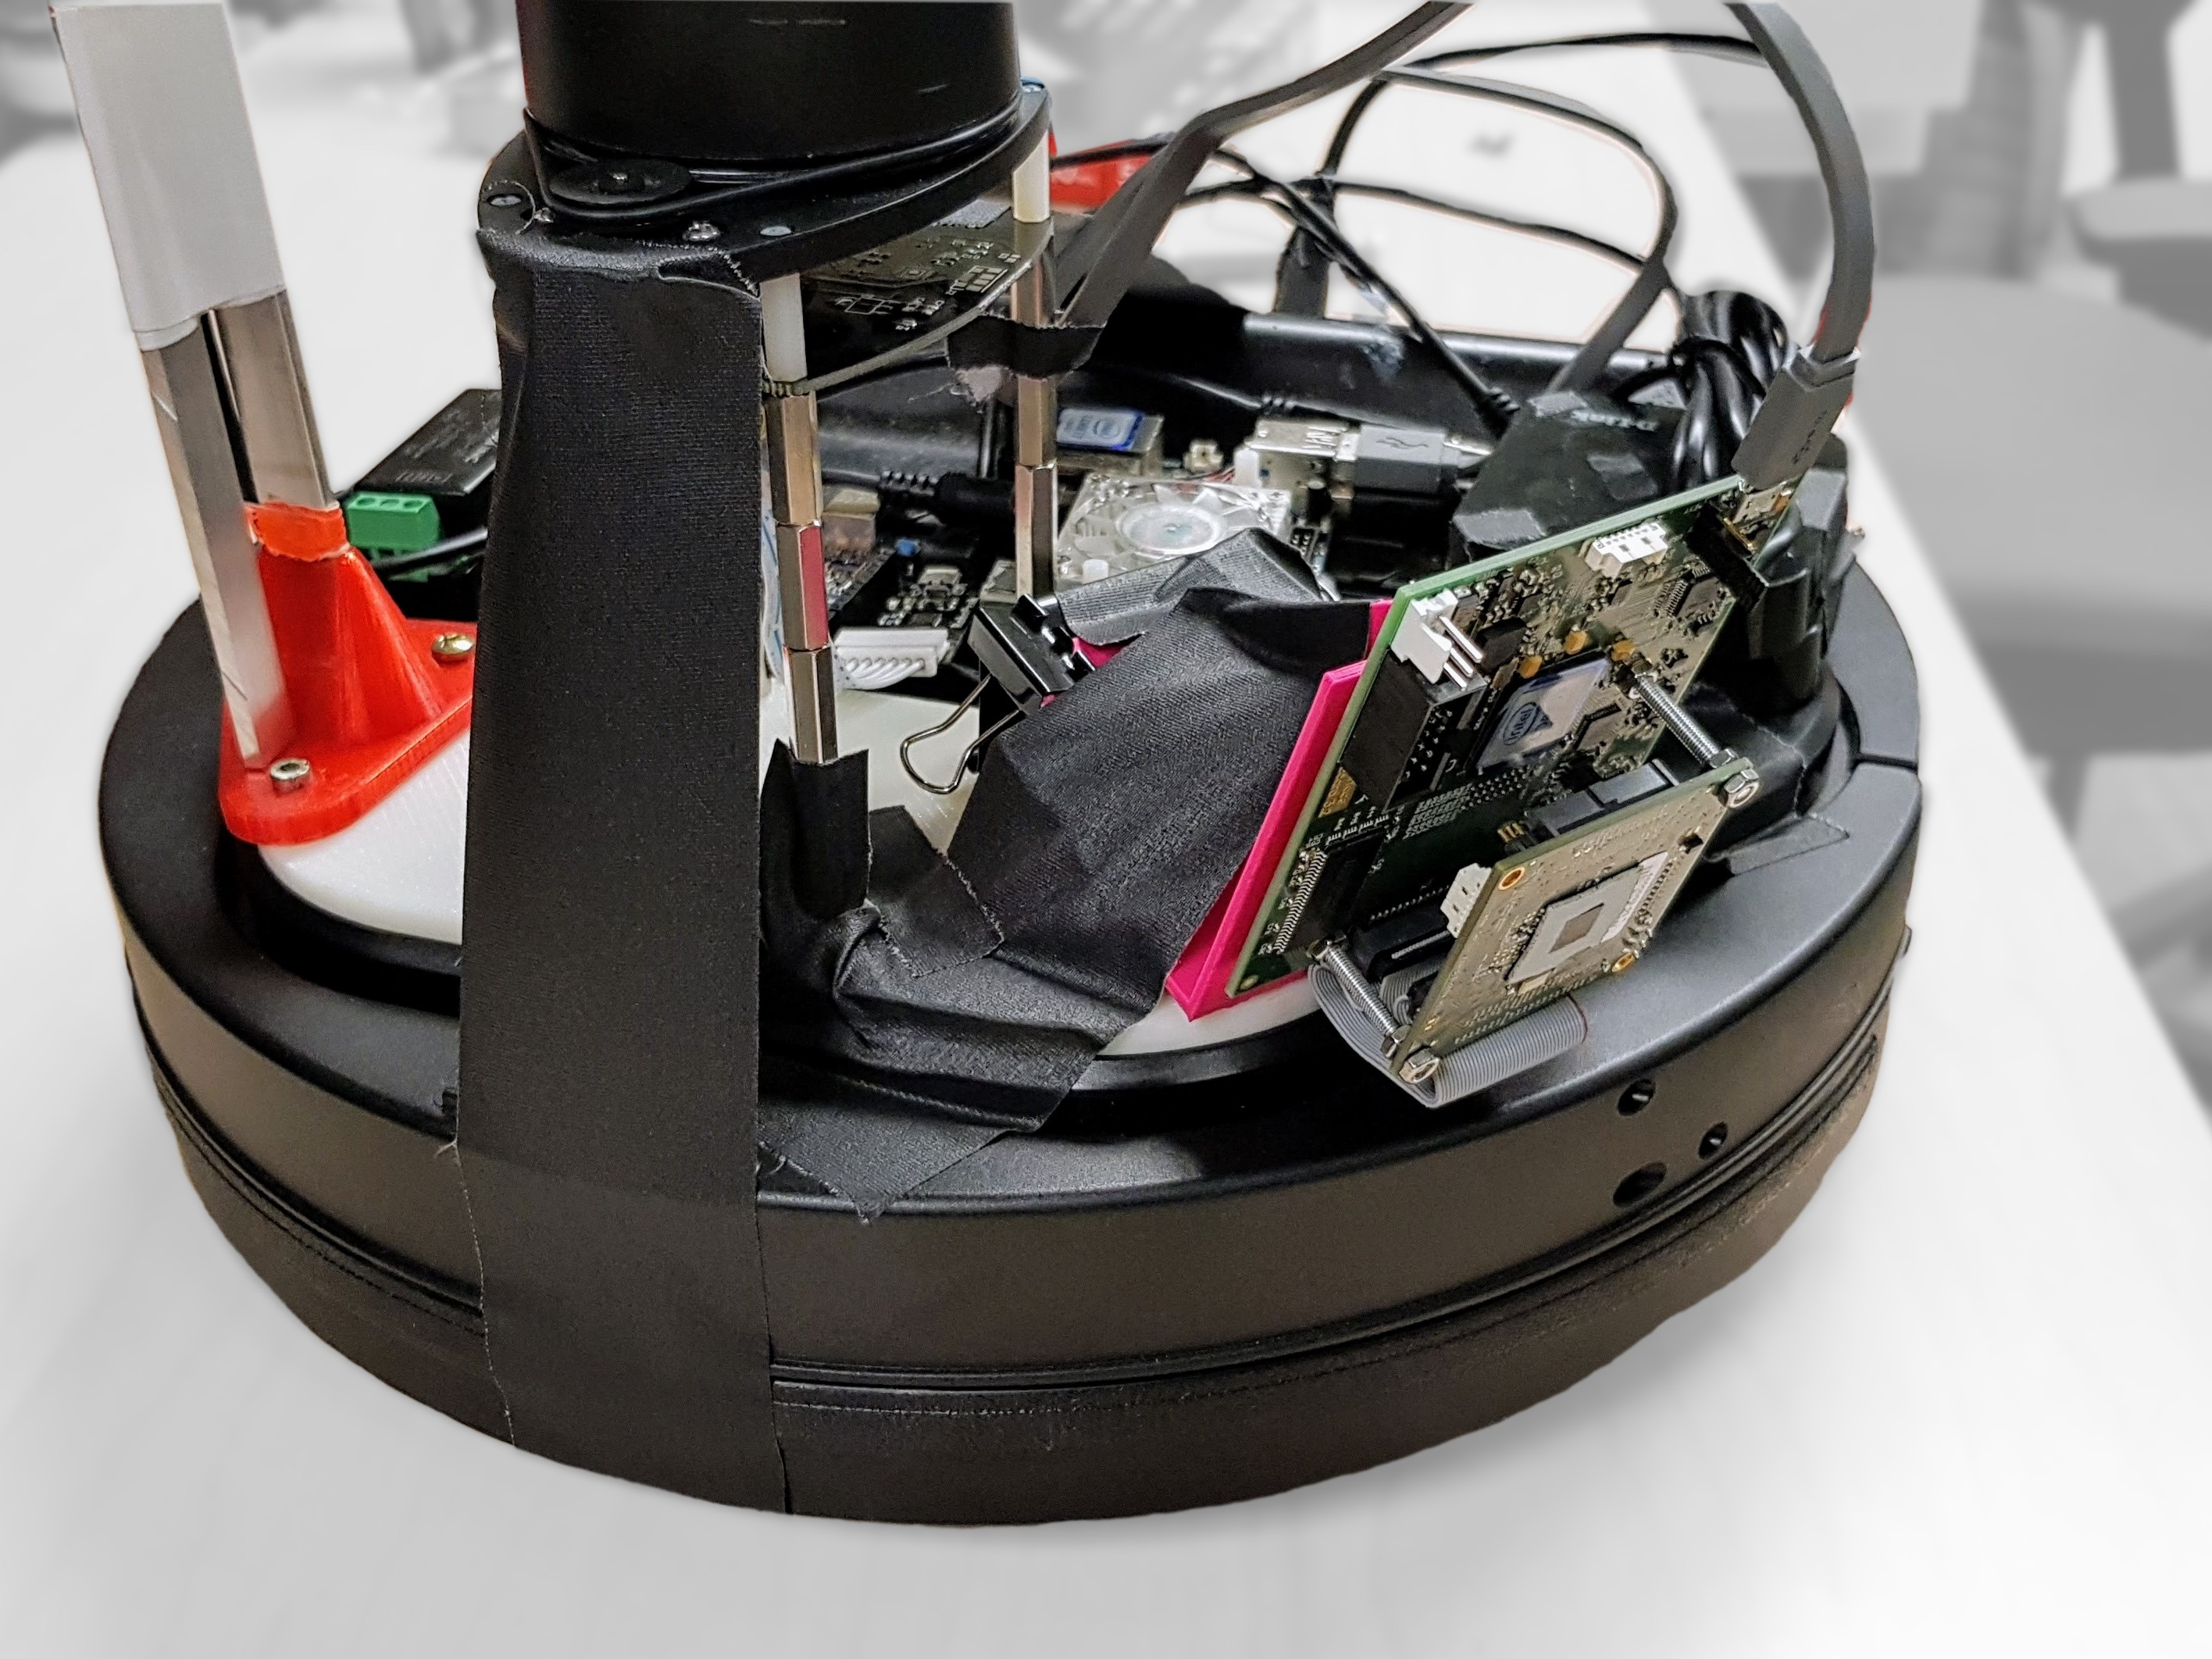
\includegraphics[width=\textwidth]{gfx/pictures/cliff_sensor}
        \caption{Sensor orientation for the Washroom scan: downward-facing vertical in an attempt to improve cliff detection}
        \label{fig:cliff_sensor}
    \end{subfigure}
\end{figure}

With scans V,W,X the negative obstacle detection capability was
analyzed in the environment shown in \cref{fig:cliff}. Cliffs, steps, and ditches are types of negative obstacles that cannot be traversed by the robot. In \cite{Jiang2015}, Jiang et al. claim that it is possible to detect this with UWB signals of various carrier frequencies. The experiments carried out for this thesis however did not show the same signal behaviour and it was not possible to reliably detect cliffs.

The Virtual Reality scan was carried out in the standard configuration
with a horizontal, slightly squinting, and not downwards angled sensor.
The assumption was that a part of the strong signal int the \SIrange{10}{20}{cm}
range were reflections from the floor, that should disappear when the
floor ends at a cliff. Visual inspection of the range profile however
shows only a extremely slight change in signal, e.g.~at cross range
\SIrange{0.8}{1.1}{m}, down range \SIrange{0.2}{0.25}{m}., where the floor could not reflect due to the radar sensor overhanging the cliff.

The Washroom scan has the sensor mounted in a vertical configuration and
downward facing (see \cref{fig:cliff_sensor}) instead to increase sensitivity to echo scattering from below. The echo intensity for cross range \SIrange{3.5}{4.5}{m} is indeed just
barely lower than \SIrange{0}{2}{m}, which matches up to where the sensor was over
the edge and over floor, respectively.

\begin{figure}[htbp]
    \centering
    \begin{subfigure}[t]{.475\textwidth}
        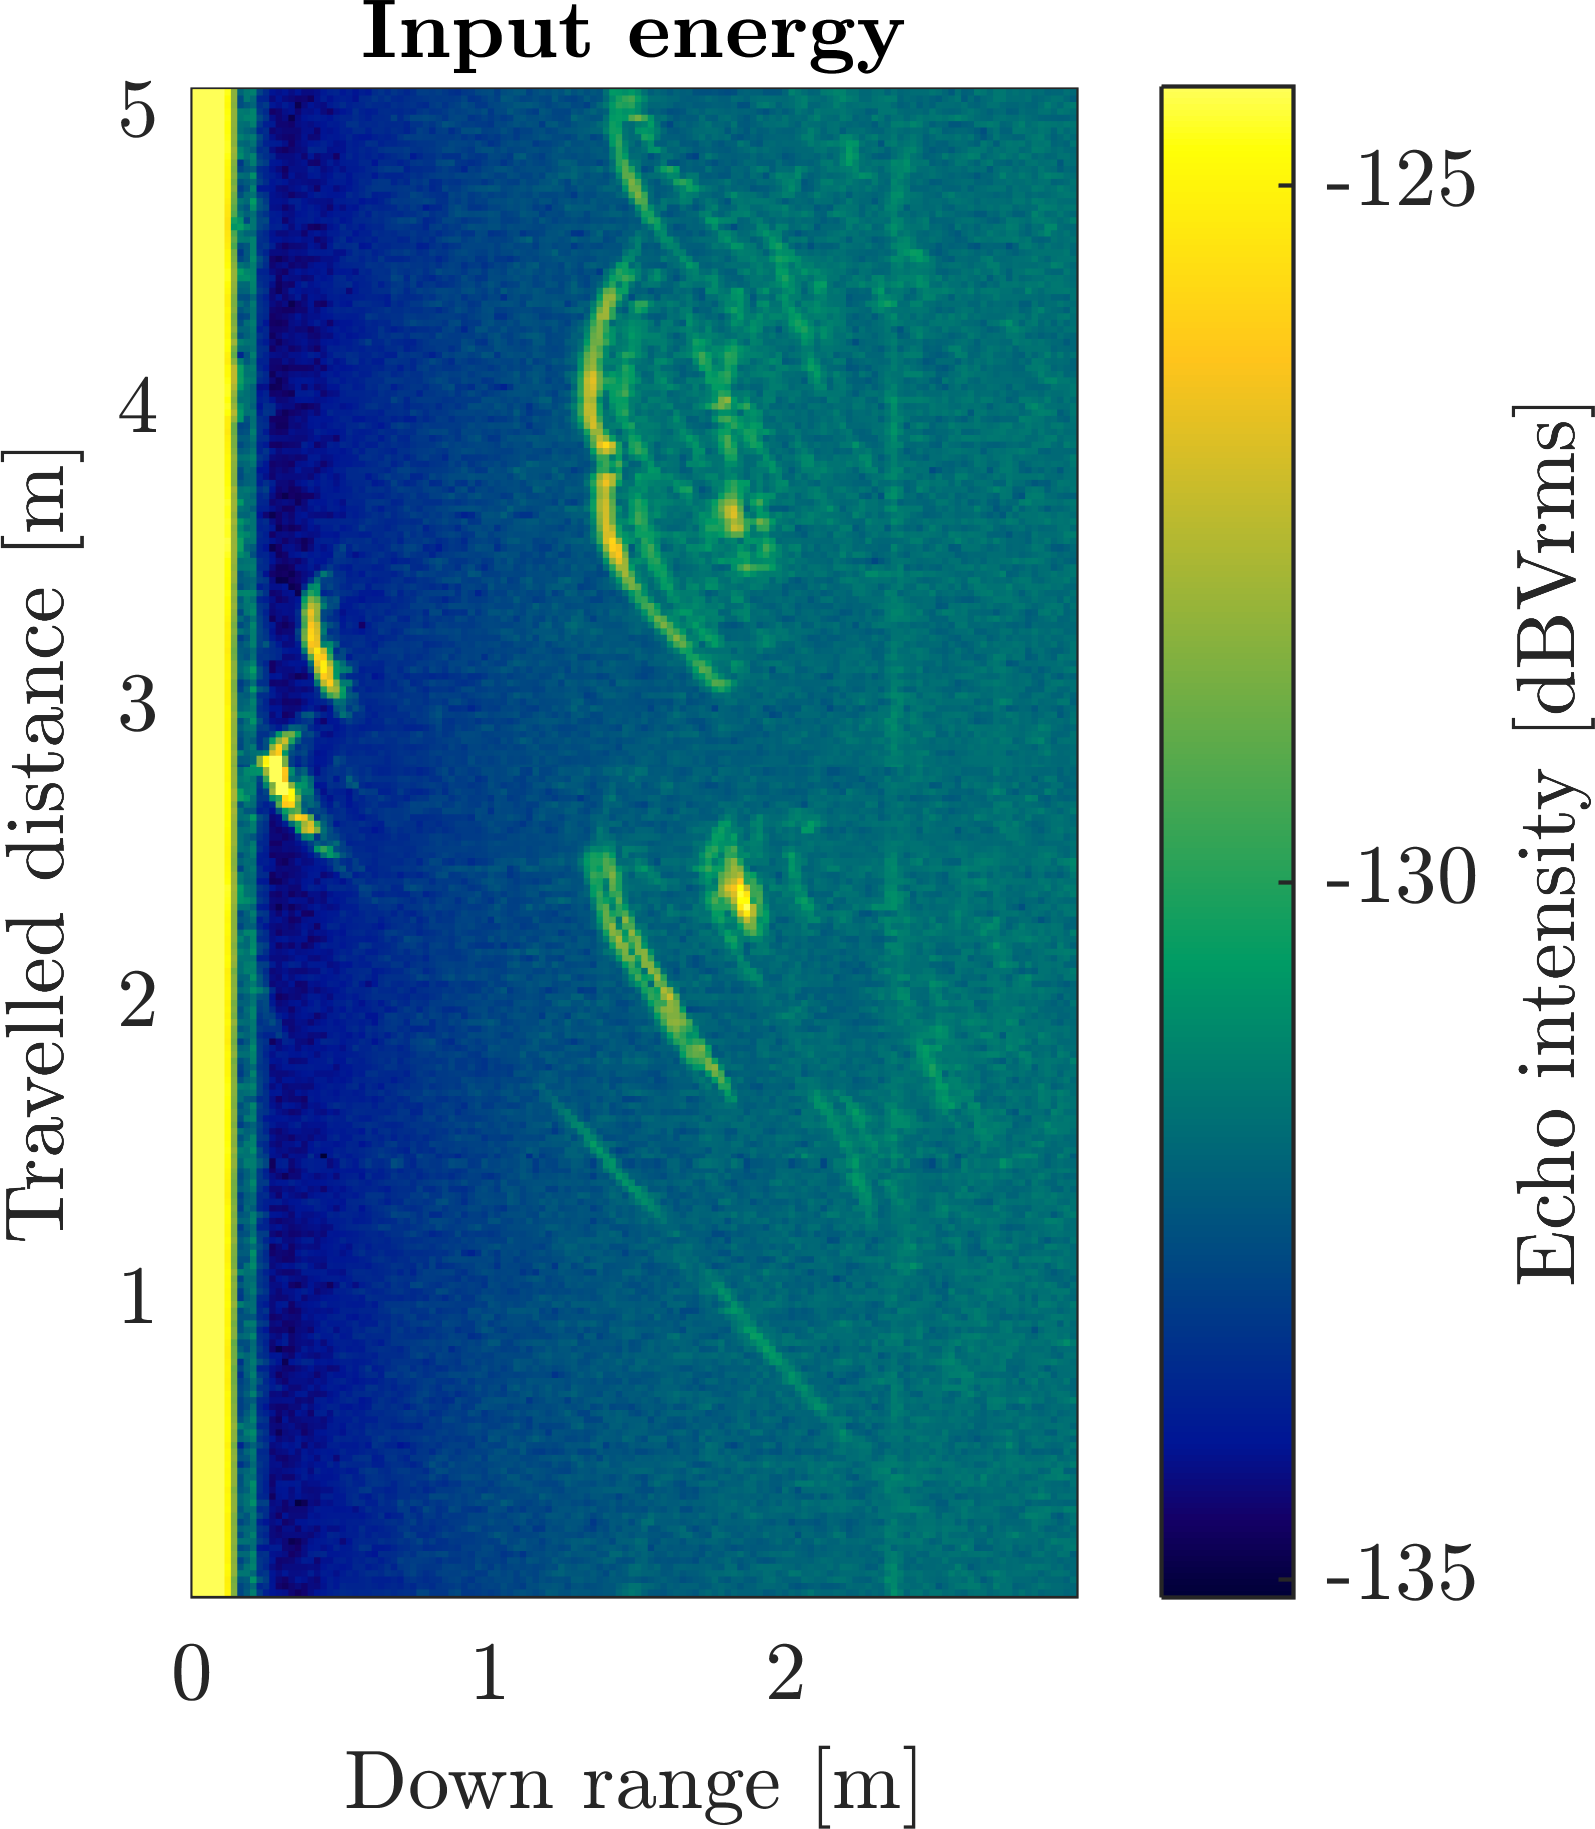
\includegraphics[max height=10cm,max width=10cm]{figures/fig_negobst}
        \caption{Regular plot.}
        \label{fig:negobst}
    \end{subfigure}%
    \hfill%
    \begin{subfigure}[t]{.475\textwidth}
        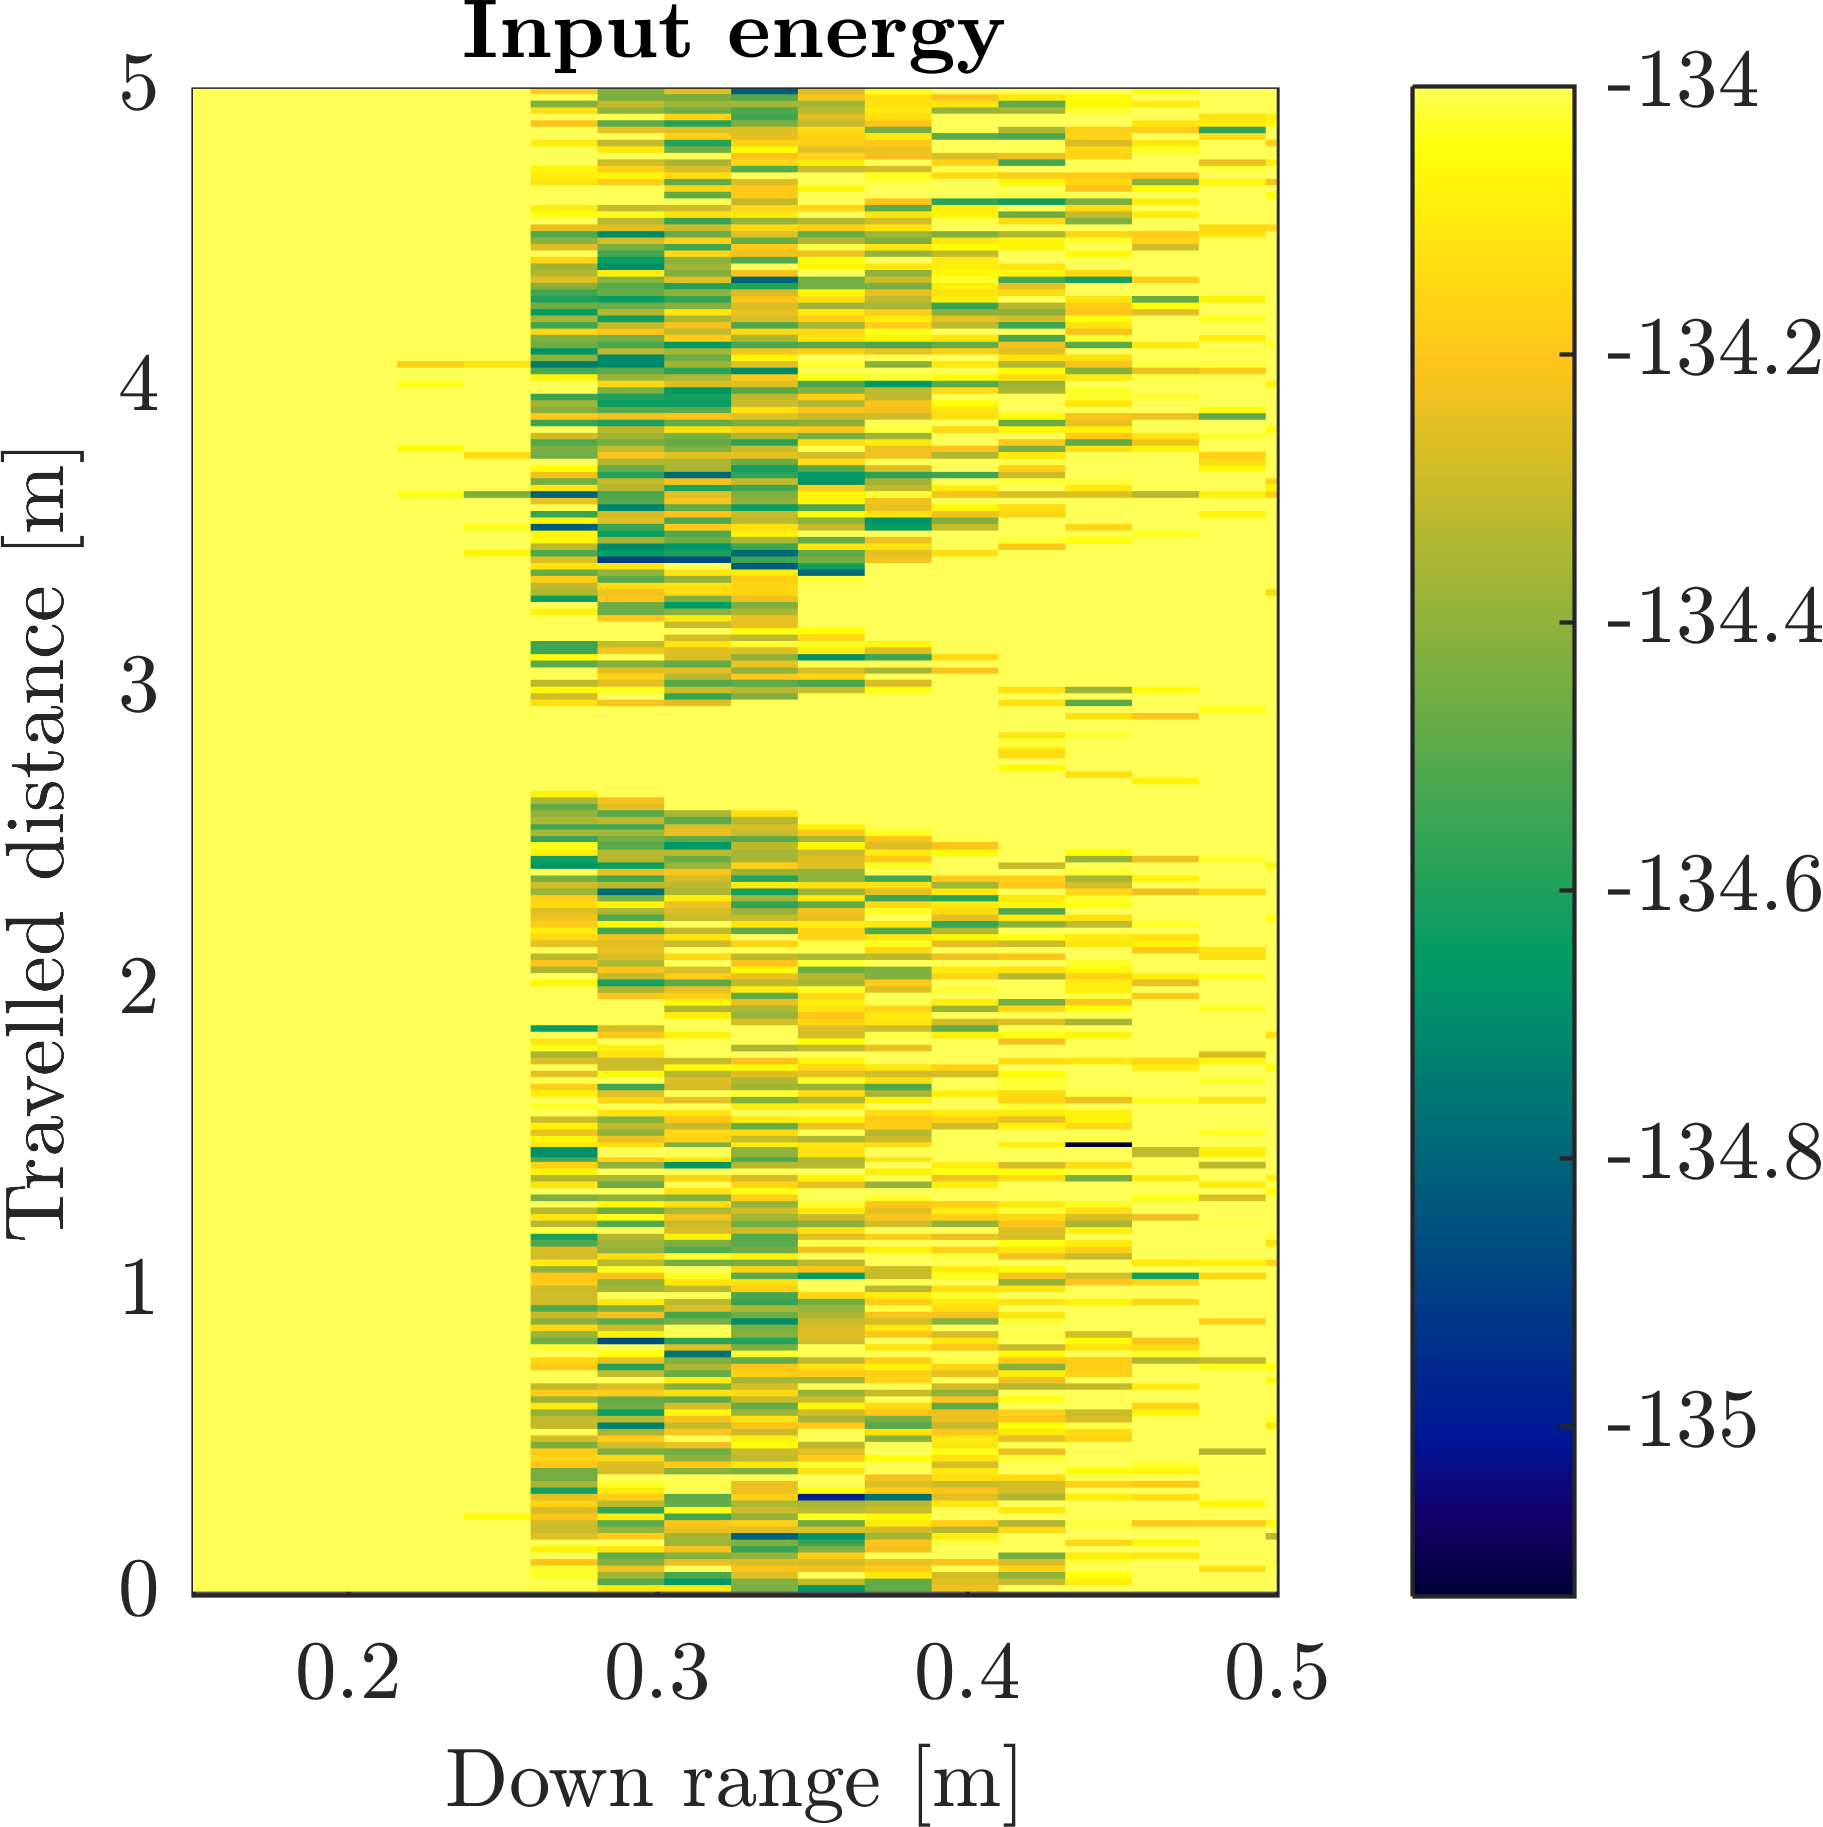
\includegraphics[max height=10cm,max width=10cm]{figures/fig_negobst_clipped}
        \caption{Zoomed and intensity-clipped for better visibility of the effect.}
        \label{fig:negobst_clipped}
    \end{subfigure}
    \caption{Input energy for the Washroom scan. Lower echo intensity at negative obstacles is hardly visible in the standard configuration.}
\end{figure}

TODO annotation-arrow pointing to darker region?

To limit the transmit crosstalk's blinding effect, the sensor was
mounted on a much higher position (on the RGBD camera mount) in the Xray
Room scan. One effects is that the robot chassis itself is constantly
visible at a distance of \SI{0.35}{cm} down range. At \SI{0.45}{cm} down range, the
floor echo is visible. There is one dip in intensity at \SI{2.5}{m} cross
range, where the sensor was not over floor. Overall the signal is
however not as conclusive as in the Washroom scan.

TODO annotation-arrow pointing to darker region?

\begin{figure}[htbp]
    \centering
    \begin{subfigure}[t]{.475\textwidth}
        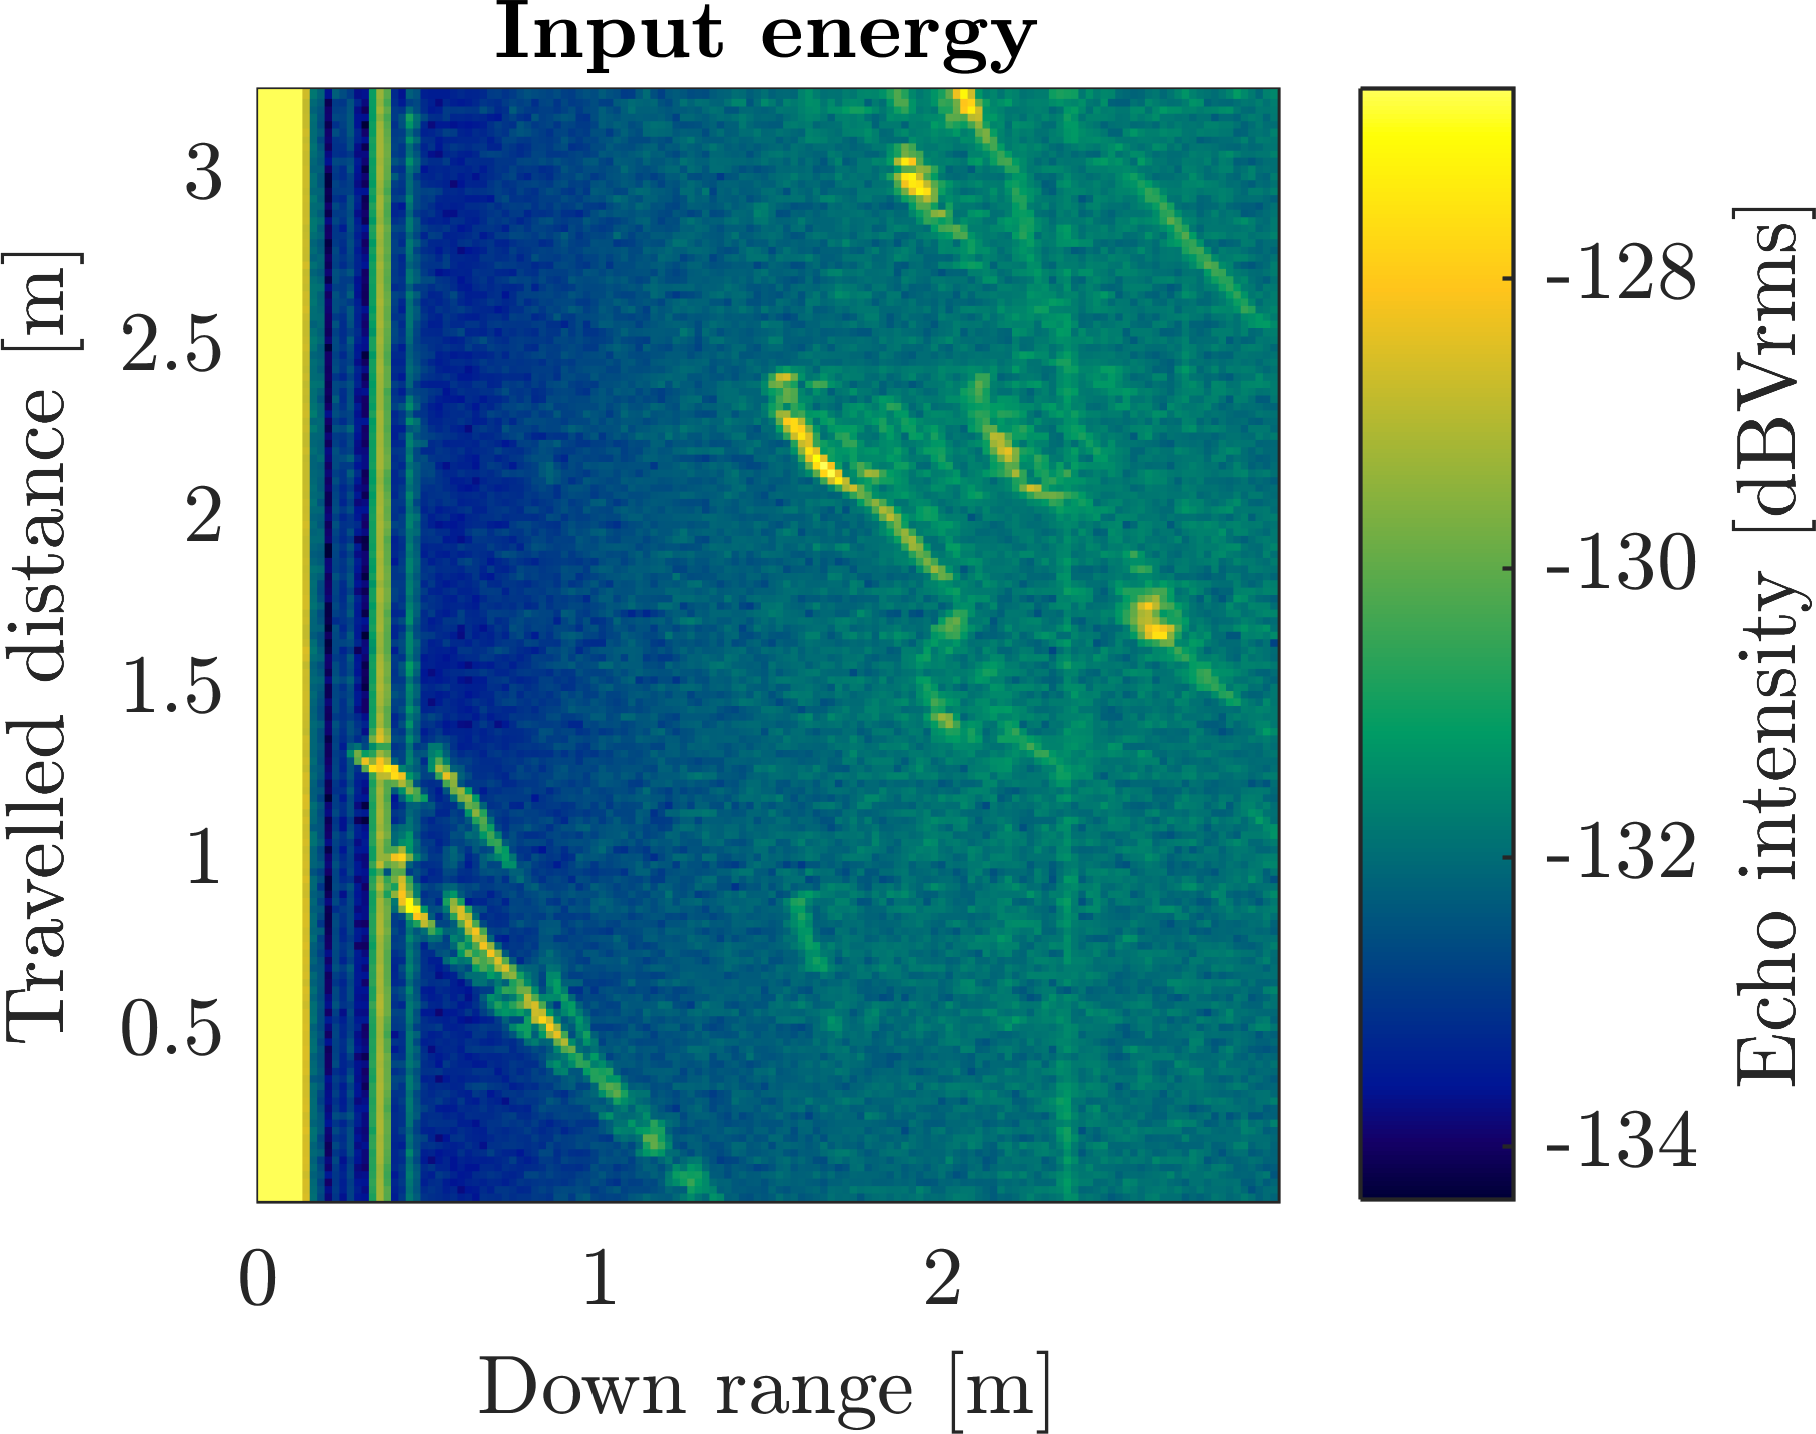
\includegraphics[max height=10cm,max width=10cm]{figures/fig_negobst_xray}
        \caption{Regular plot.}
        \label{fig:negobst_xray}
    \end{subfigure}%
    \hfill%
    \begin{subfigure}[t]{.475\textwidth}
        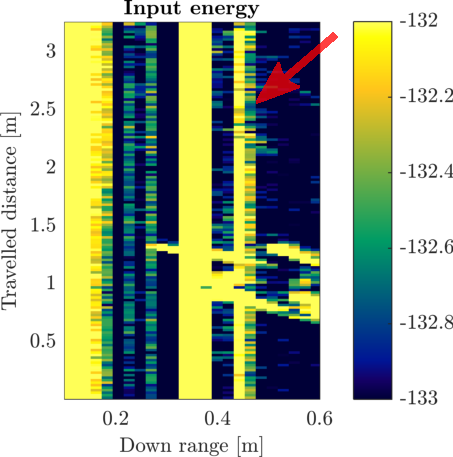
\includegraphics[max height=10cm,max width=10cm]{figures/fig_negobst_xray_clipped}
        \caption{Zoomed and intensity-clipped for better visibility of the effect.}
        \label{fig:negobst_xray_clipped}
    \end{subfigure}
    \caption{Input energy for the XRay Room scan. Negative obstacles effect is not better with a higher-mounted vertical configuration.}
\end{figure}


Maybe the signal could be improved with improved background subtraction
(see \#REF). However, the three scans show that it is very hard to
detect negative obstacles with this sensor. A radar sensor of this type
will hence not be a viable replacement for regular cliff detection
sensors like the floor facing infrared distance sensors in the Kobuki
base.

\subsection{Cable detection}\label{cable-detection}

Cables on the floor are another interesting target that falls into the
category of obstacles being a very common occurrence in the real world,
but are hard to detect with conventional obstacle sensors. The Y (Is
There A Cable On The Floor) scan deals with the detection if this kind
of obstacle. For this, the same camera-mounted vertical configuration as
in X Ray Room was used. Again, there is a constant robot chassis echo at
down range \SI{0.35}{m}. As the robot is driving closer towards the power cable
on the floor, the cable's echo is visibly coming closer before it
disappears under the robot's chassis. The echos at \SI{0.9}{m} down range show
the two can towers at the end of the cable.

\begin{figure}[htp]
    \centering
    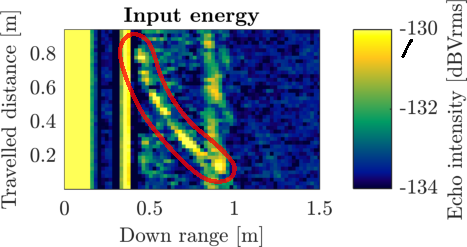
\includegraphics[max height=10cm,max width=10cm]{figures/fig_cable}
    \caption{Input energy of the Y (Is There A Cable On The Ground) scan. The center arc represents the echo of a cable on the floor as the robot approaches.}
    \label{fig:cable}
\end{figure}

Both the X Ray Room and Y (Is There A Cable On The Floor) introduce a
new geometry that lifts the radar sensor out of the two dimensional
mapping plane. The geometry is better described with a 3D case, for
which more than

\subsection{Minimum distance}\label{minimum-distance}

The constant noise from the transmission crosstalk leads to a high
minimum detection distance as explained in \#REF. The effect is that
targets can not be projected onto the map if the robot is too close to
them. This is an issue in the Sauna scan, where the Glass wall right at
the beginning of the robot path cannot be mapped in its entirety.



%%%%%%%%%%%%%%%%%%%%%%%%%%%%%%%%%%%%%%%%%%%%%%%%%%%%%
\section{Comparison with other mapping techniques} \label{comparison-with-other-mapping-techniques}

While some of the radar reprojection maps speak for themselves, they
make more sense when compared to other mapping techniques. In the
following, SAR techniques, Laser slam, and RGBD slam are compared to the
radar reprojection.

\subsection{SAR}\label{sar-1}
Synthetic aperture radars make a lot of sense in other applications
where the radar is moved over or through a map. The big difference to
this application is that ``professional'' SAR applications have radar
sensors that sit in vehicles that are not in the mapping plane.
Airplanes, satellites and even Submarines scan the earth like that.

There are a few examples for UWB radars being moved sideways (usually on a rail) in an effort to scan a scene with synthetic aperture radar.
Gregory L. Charvat's ``tin can'' radar \cite{Charvat2014} might be the most famous one, with many examples at \url{http://glcharvat.com/shortrange/}.
Another great resource was Henrik Forstén's Homemade Synthetic Aperture
Radar, documented in \cite{Forsten2015} (see \cref{fig:forsten}). He used an Omega-k algorithm \cite{Tolman2008} and Stolt interpolation \cite{Cumming2004} to correct the range migration arcs.

\begin{figure}
% 0.95 * 3264*817/2448 / (3264*817/2448 + 1299) = 0.43330076762
% 0.95 * 1299 / (3264*817/2448 + 1299) = 0.51669923238
    \begin{subfigure}[t]{0.43330076762\textwidth}
        \centering
        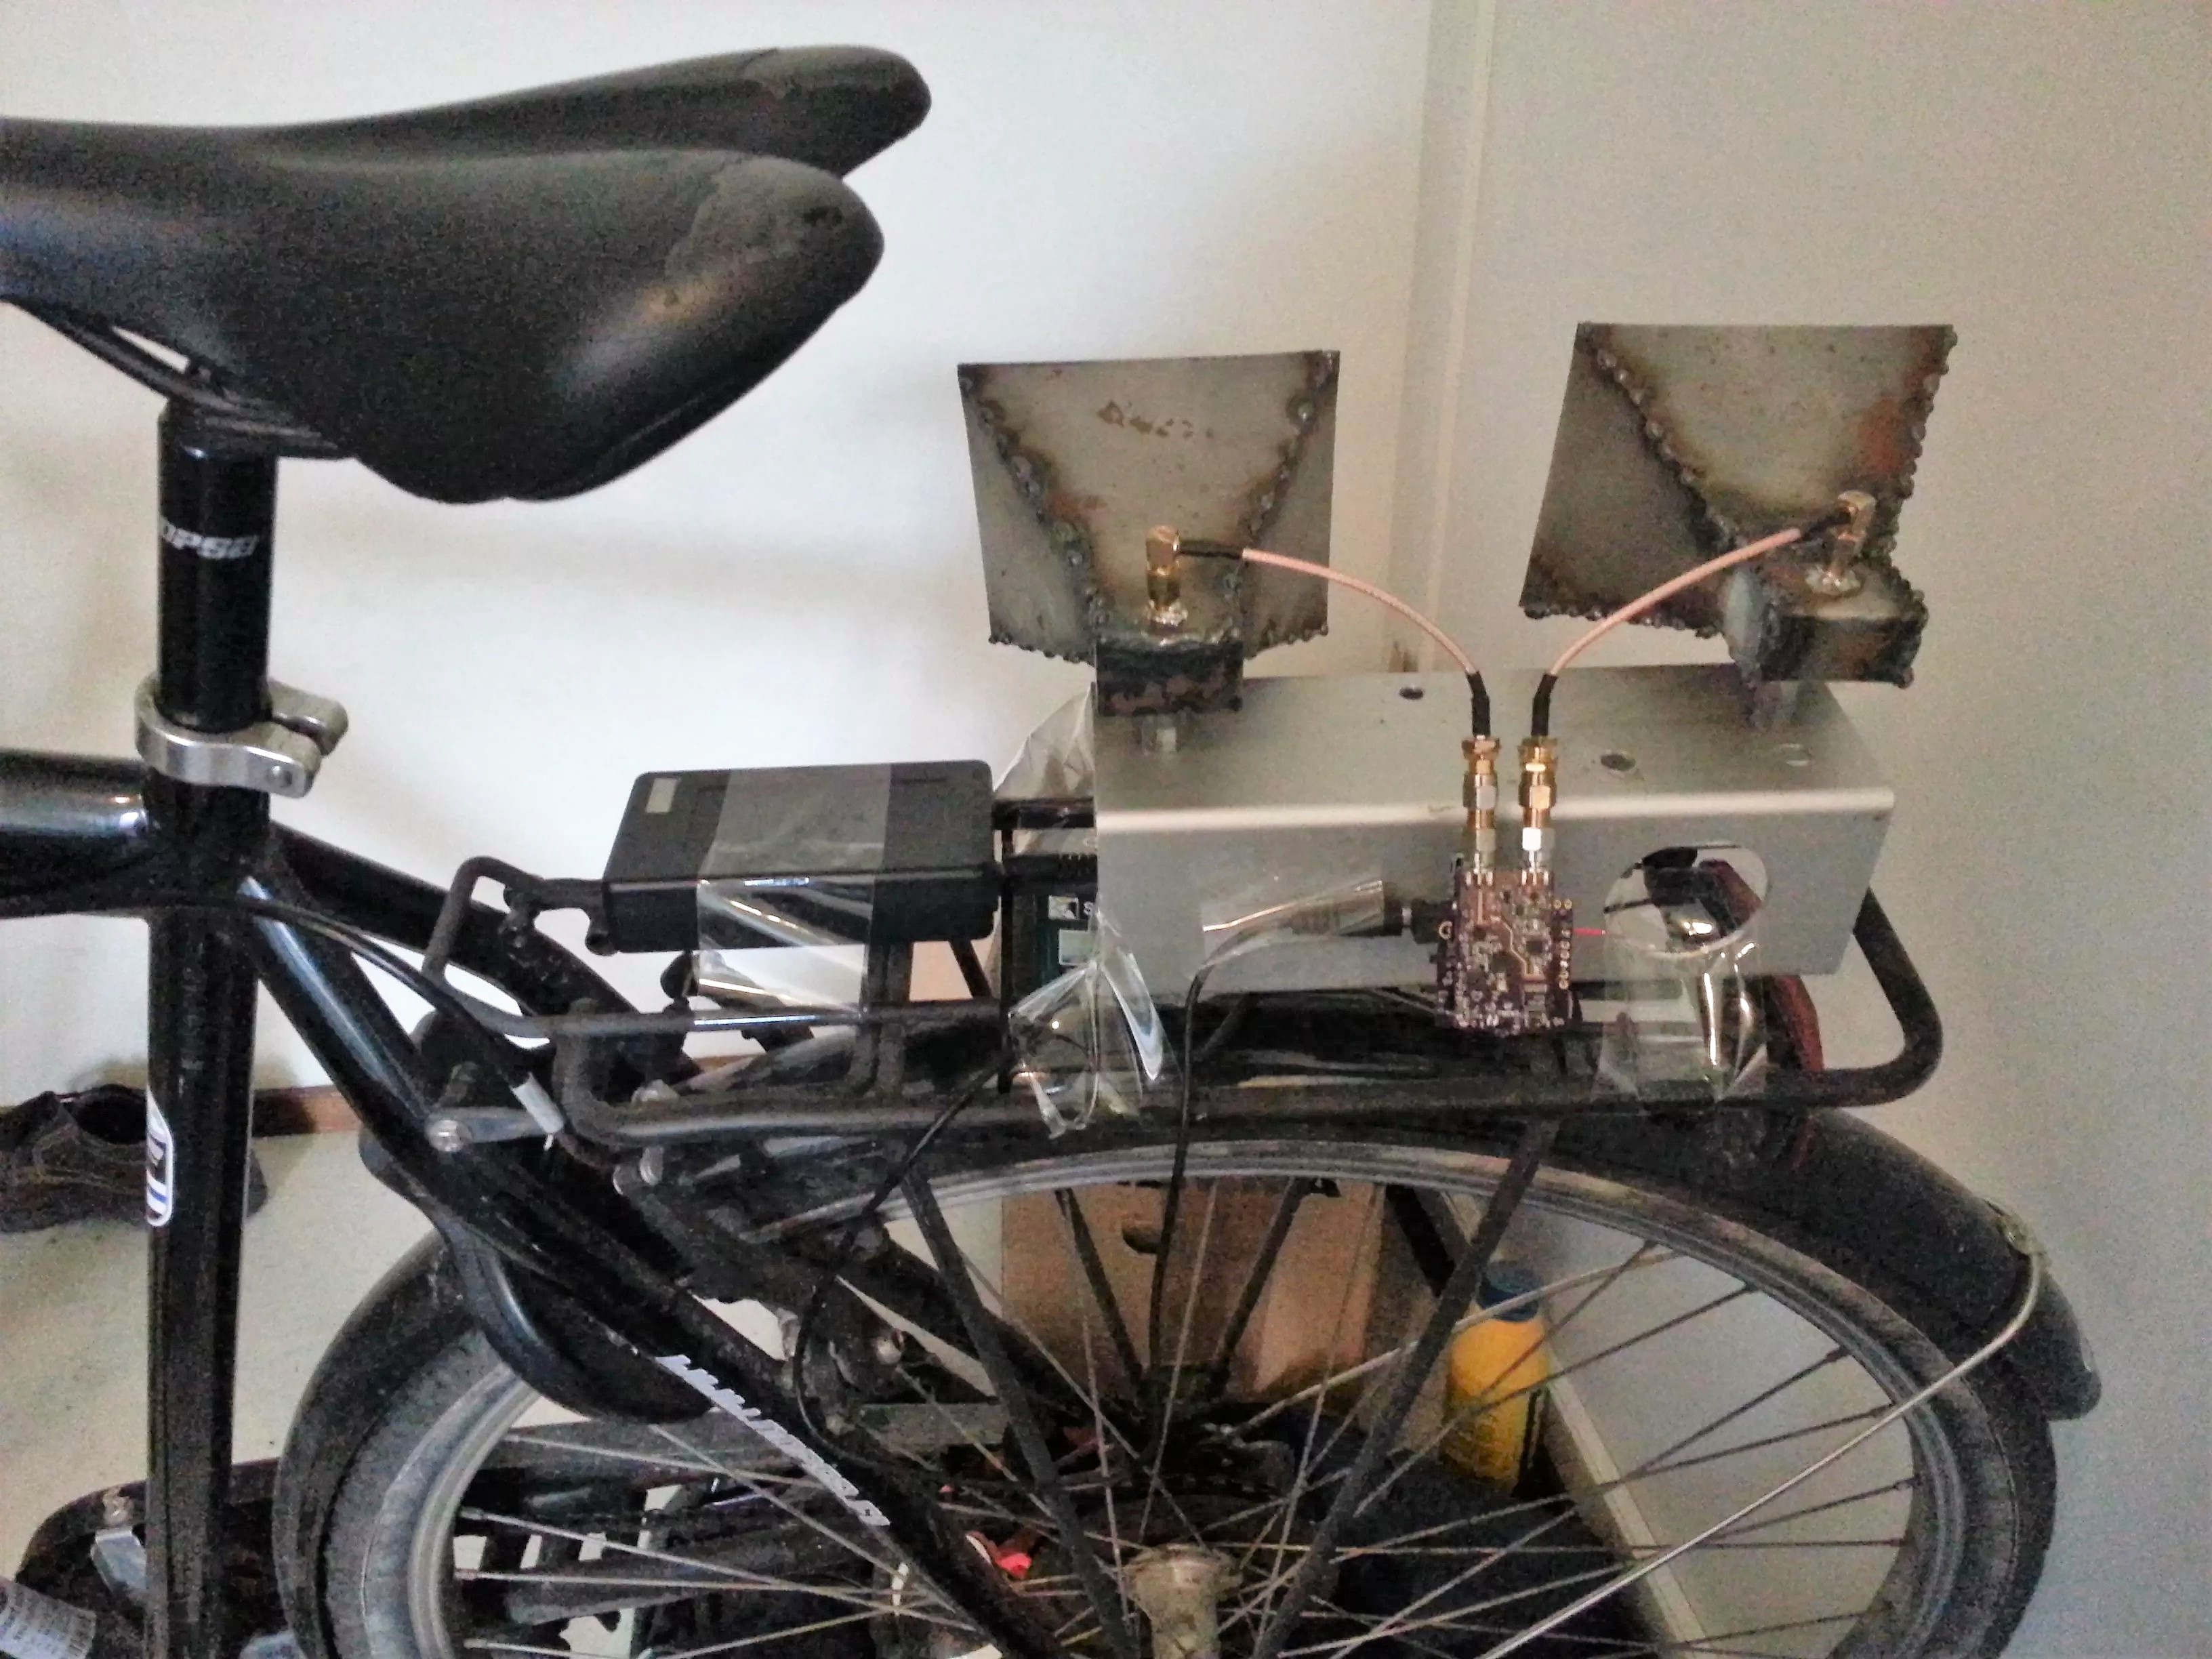
\includegraphics[max width=\linewidth]{gfx/pictures/forsten_1.jpg}
        \caption{Forstén's SAR setup. Source: \cite{Forsten2015}}
        \label{fig:forsten_1}
    \end{subfigure}%
    \hfill%
    \begin{subfigure}[t]{0.51669923238\textwidth}
        \centering
        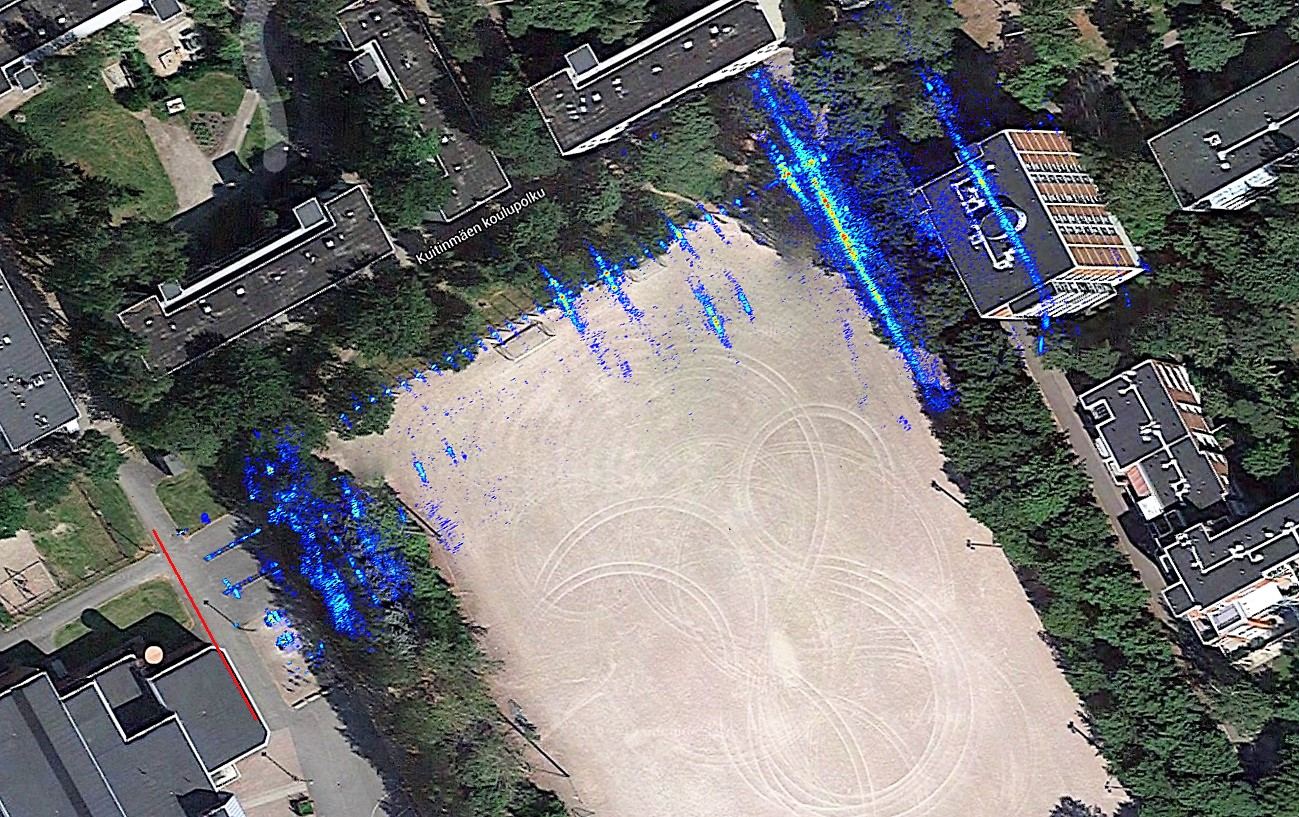
\includegraphics[max width=\linewidth]{gfx/pictures/forsten_2.jpg}
        \caption{Forstén's SAR imagery agrees well with aerial imagery. Source: \cite{Forsten2015}}
        \label{fig:forsten_2}
    \end{subfigure}
    \caption{After omega-k processing and autofocusing, Forstén's synthetic aperture radar can create nice-looking broadside SAR imagery.}
    \label{fig:forsten}
\end{figure}


Forstén was able to greatly improve his data quality by use of an minimum-entropy based auto-focusing algorithm. The trick with this is that the radar needs to move in a very straight line, where the ``error in path linearity should be around less than tenth of a wavelength'' \cite{Forsten2015}. In Forstén's radar, this is about \SI{5}{mm}. However with the \SI{60}{GHz} Omniradar this is around \SI{0.5}{mm}. Keeping a straight line with less than half a millimeter of linearity error is not realistically achievable on the Kobuki platform.

One big inherent problem with synthetic aperture radar algorithms is
that basically all of them assume the radar to move in a straight line.
While changing the squint angle helps to deal with issues such as earth
curvature in satellite applications, SAR with curved or even arbitrary
paths is a challenging topic, particularly because auto-focusing, which
again relies on phase information, becomes more difficult
\cite{Axelsson2002}.

\subsection{RGBD}\label{rgbd-1}
The Kobuki robot was also carrying an Astra Orbbec Mini\footnote{\url{https://orbbec3d.com/astra-mini/}} strutured light depth camera. Using the Rtabmap \cite{Labbe2014} ROS package\footnote{\url{http://wiki.ros.org/rtabmap_ros}}, some 3D scans of the office environment where made. \cref{traditional-obstacle-sensors} already showed the shortcomings of lidar and RGBD sensors, but in this section the same \cref{fig:lidar_rgbd2,fig:rgbd_glasswall2} are compared with radar reprojection.

\begin{figure}
    \begin{subfigure}[t]{.485\textwidth}
        \centering
        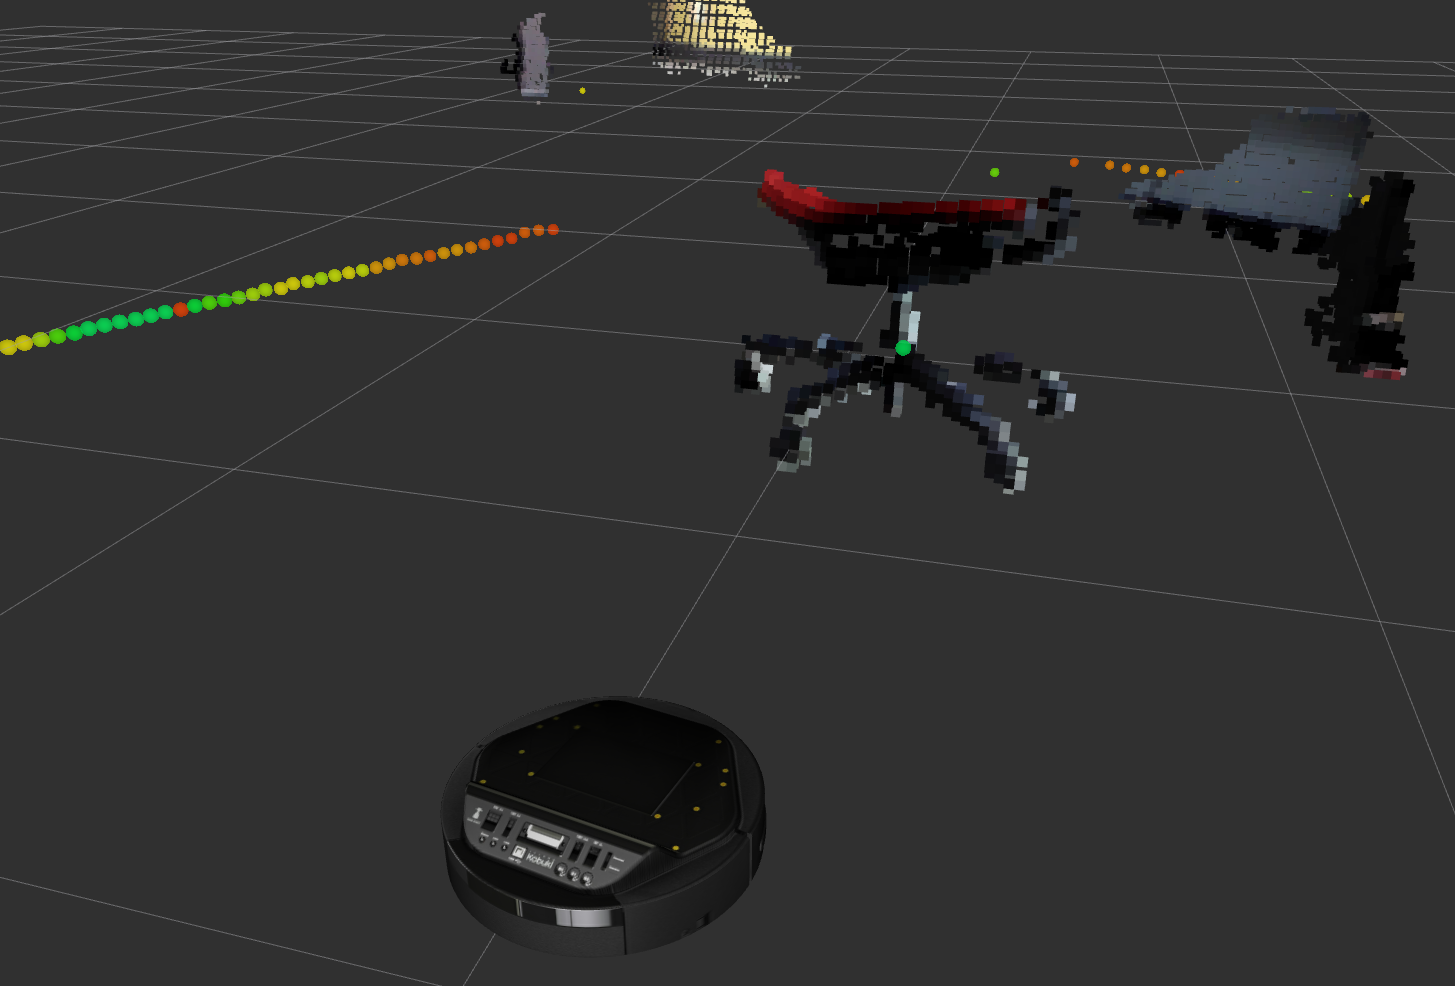
\includegraphics[max width=\textwidth]{gfx/screenshots/chair_laser_vs_rgbd}
        \caption{Laser fails to detect horizontal chair legs.}
        \label{fig:lidar_rgbd2}
    \end{subfigure}%
    \hfill%
    \begin{subfigure}[t]{.485\textwidth}
        \centering
        \def\svgwidth{\linewidth}
        \input{gfx/screenshots/rgbd_glasswall.pdf_tex}
        \caption{RGBD camera can not detect glass surface.}
        \label{fig:rgbd_glasswall2}
    \end{subfigure}%
    \caption{RViz screenshots showing traditional sensor shortcomings.}
\end{figure}

\Cref{fig:chairlegs} shows clearly that the radar reprojection contains horizontal chair legs, while the lidar scan does not. The scene in \cref{fig:rgbd_glasswall2} matches with the Underground scan, where the glass wall is clearly visible.

\begin{figure}
    \begin{subfigure}[t]{.485\textwidth}
        \centering
        \includegraphics[max width=\textwidth]{gfx/pictures/torturechamber_scene}
        \caption{View of the Torturechamber scan environment. Blue path is the robot's path.}
        \label{fig:chairs_scene}
    \end{subfigure}%
    \hfill%
    \begin{subfigure}[t]{.485\textwidth}
        \centering
        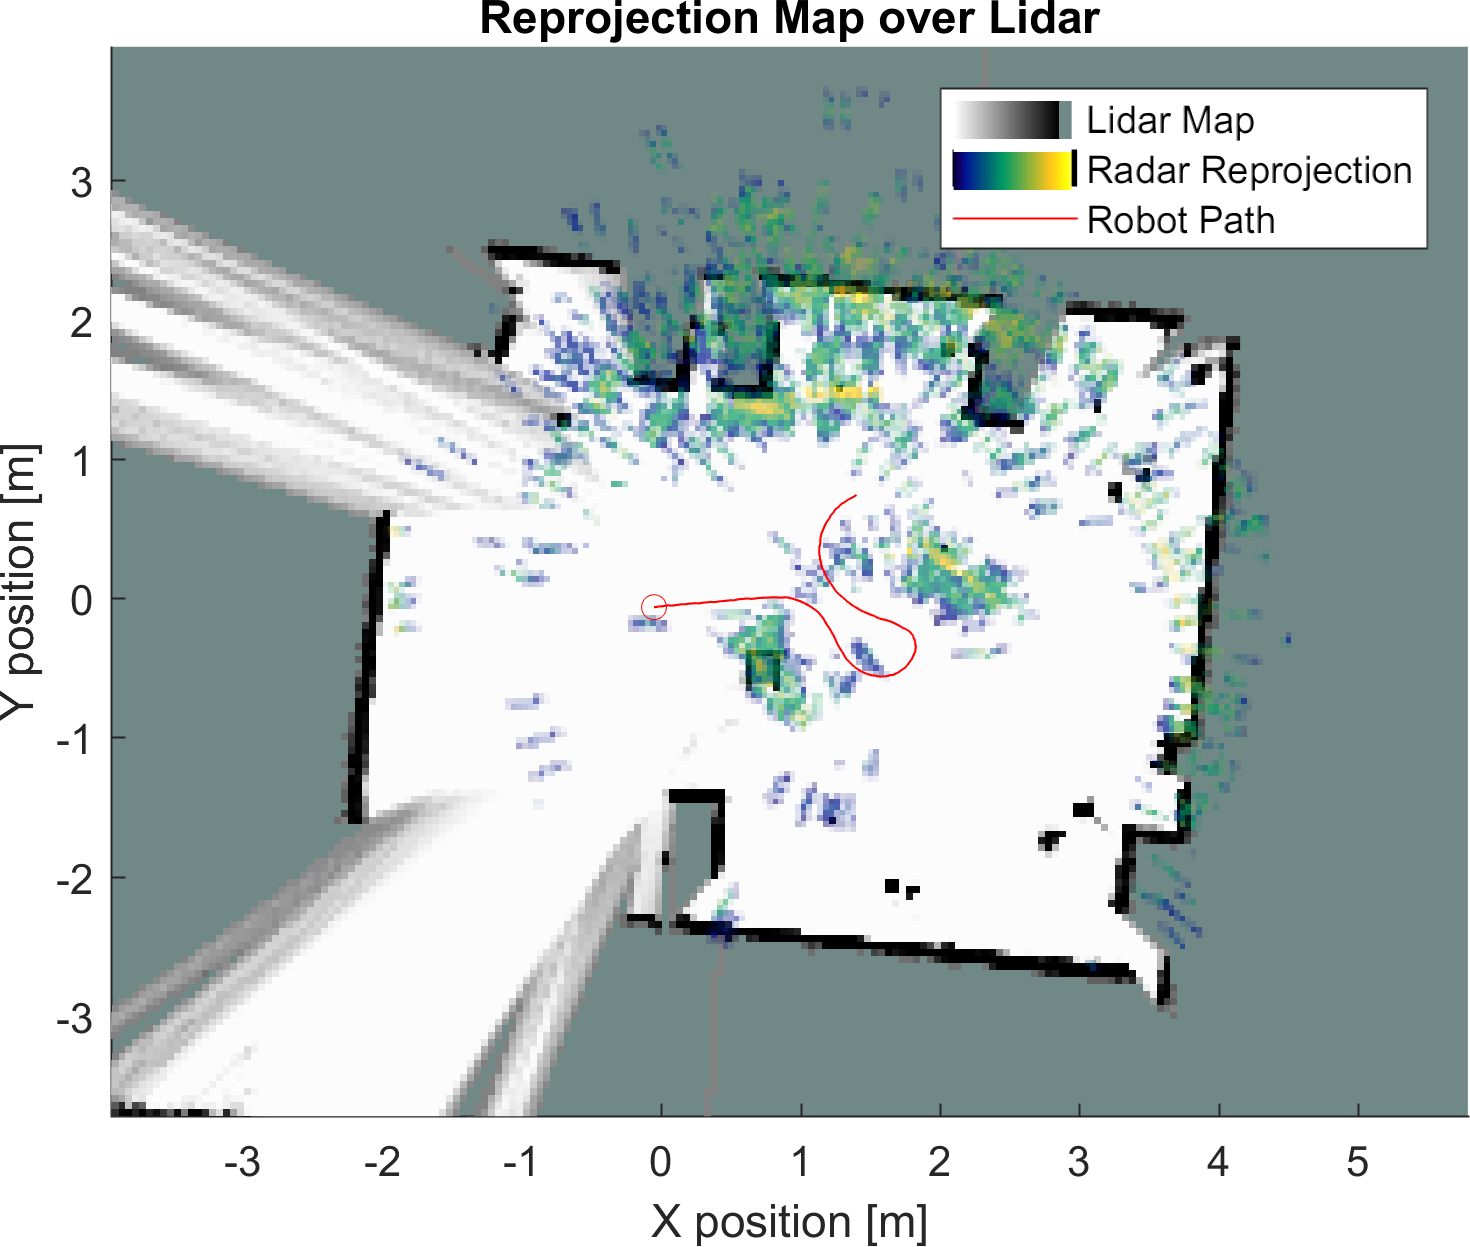
\includegraphics[max width=\textwidth]{gfx/results/torturechamber_map}
        \caption{Torturechamber reprojection map over lidar slam gridmap.}
        \label{fig:chairs_map}
    \end{subfigure}%
    \caption{In the Torturechamber scan, horizontal chair legs are visible in the reprojection map but not in the lidar scan.}
    \label{fig:chairlegs}
\end{figure}

\subsection{Lidar}\label{lidar-1}
As stated in \cref{kobuki}, the Kobuki robot used in the experiments was equipped with an RPLidar and a computing platform powerful enough to perform slam. Lidar slam is the go-to, standard approach when it comes to mapping the environment around a robot. After years of research and product development, even relatively cheap lidar systems like the RPLidar have acceptable range resolution. While they can't provide ground truth data (see problems with lidar data in \cref{traditional-obstacle-sensors}), it makes sense to compare the radar reprojection maps with laser scan maps. This is why all scans after Mancave have lidar maps associated.
%TODO!
Not that there is a bug in the rosbag to Matlab conversion that sometimes causes the complete map to be rotated against the lidar map by some degrees.
